\chapter{Backend}
Für die entwickelte Anwendung kommt die Plattform \glqq Firebase\grqq{} von Google zum Einsatz.
\\
Diese stellt neben einer Echtzeit-Datenbank, Authentifizierungs-Funktionen und Cloud-Messaging, auch Speicherplatz sowie ein Hosting für Web-Apps zur Verfügung.In der Basis-Version, welche auch für die Entwicklung der vorliegenden Anwendung verwendet wurde, ist die Nutzung kostenlos. Für höhere Leistungsansprüche stehen kostenpflichtige Pakete zur Verfügung.Im nachfolgenden erfolgt eine Erläuterung der einzelnen Komponenten, die von der Anwendung benutzt werden.

\section{Echtzeit-Datenbank}
Bei der von Firebase verwendeten Datenbank handelt es sich um eine sogenante NoSQL-Datenbank. Im Gegensatz zu anderen Datenbank-Systemen wie beispielsweise MySQL, erfolgt die Abspeicherung der Daten dokumentenbasiert im JSON-Format.
Dokumentenbasiert bedeutet, dass einzelne Einträge der Datenbank als Objekte abgelegt werden. Die Objekte sind von Grund auf nicht an Schemata gebunden und können beliebige Strukturen beinhalten.
Dabei können auch Objekte, die von ihrer Gruppierung her gleich sind, unterschiedlich viele und anders typisierte Daten beinhalten.\\

\section{Organisation}
Die Benennung der Gruppen von Datensätzen ist von Firebase sehr flexibel gestaltet und ermöglicht beliebige Namen.

Es existieren folgende drei Gruppen:
\begin{itemize}
\item bookings (Abbildung \ref{backend_database_bookings})
\item customers (Abbildung \ref{backend_database_customers})
\item resources (Abbildung \ref{backend_database_resource})
\end{itemize}

\begin{figure}[H]
    \centering
    \begin{minipage}[t]{0.32\linewidth}
        \centering
        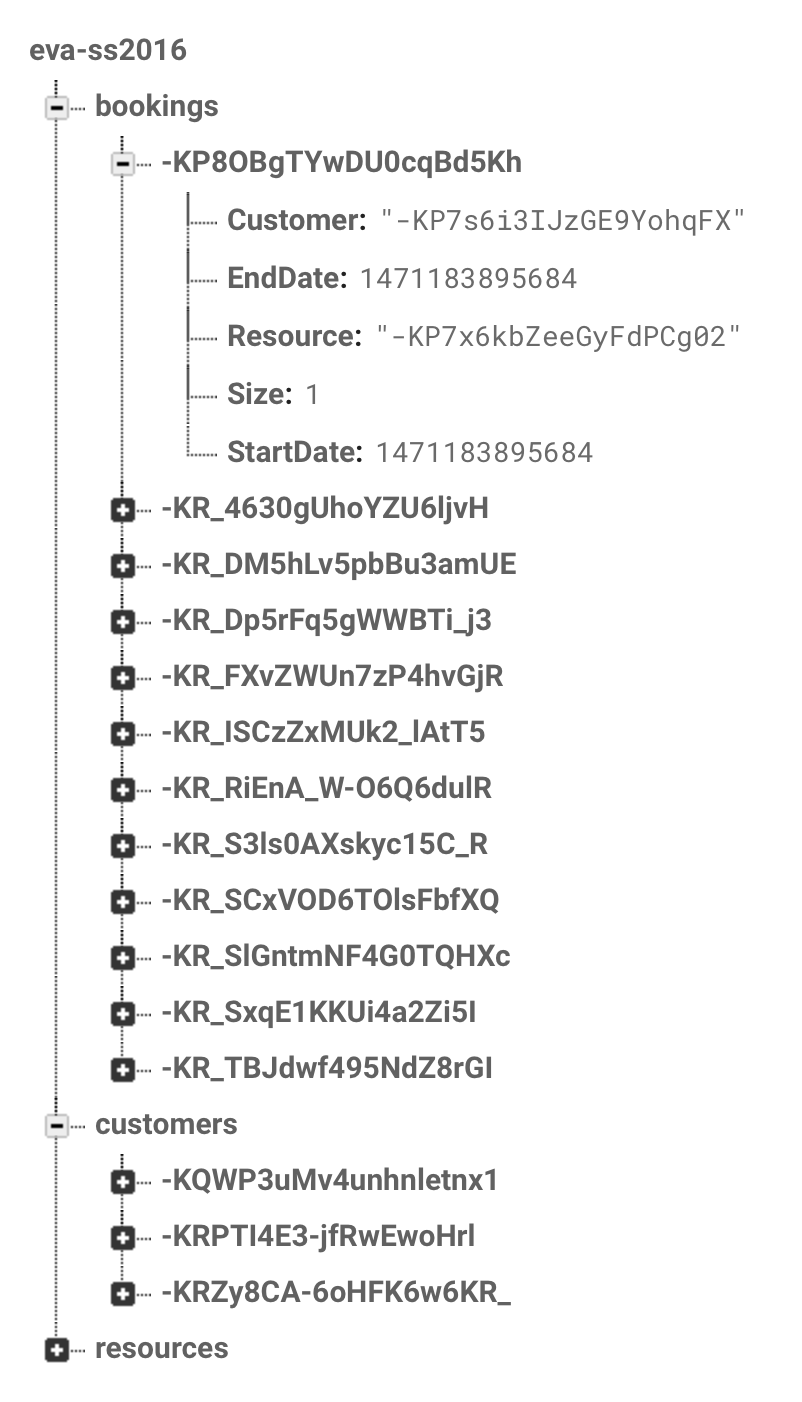
\includegraphics[width=\linewidth]{images/backend_database_bookings.png}
        \caption{Datenbank Buchungen}
        \label{backend_database_bookings}
    \end{minipage}% <- sonst wird hier ein Leerzeichen eingefügt
    \hfill
    \begin{minipage}[t]{0.32\linewidth}
        \centering
        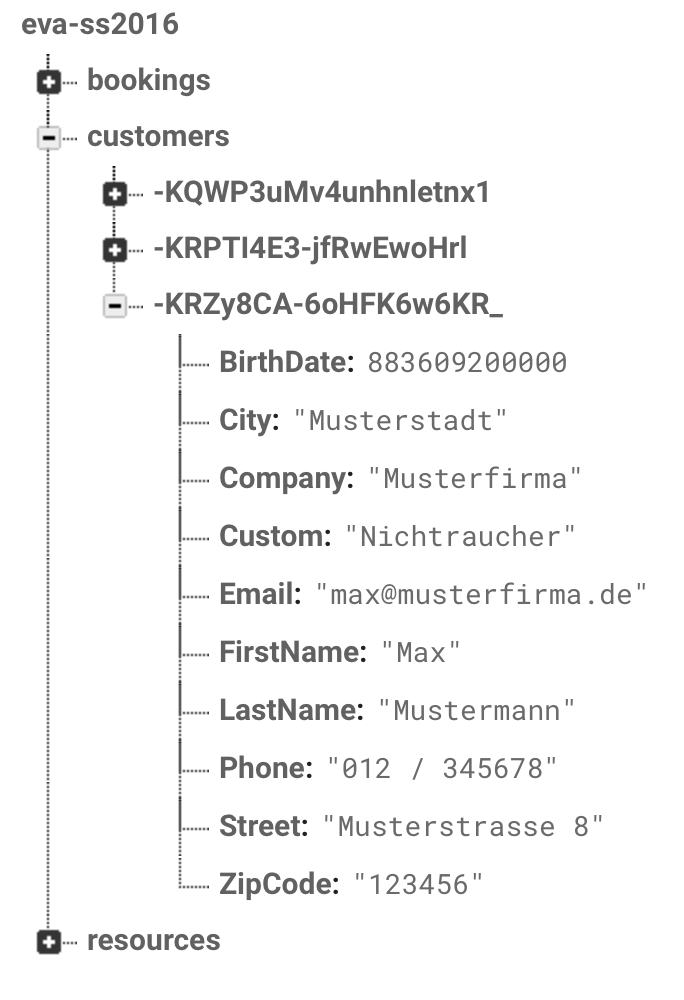
\includegraphics[width=\linewidth]{images/backend_database_customers.png}
        \caption{Datenbank Kunde}
        \label{backend_database_customers}
    \end{minipage}
    \hfill
    \begin{minipage}[t]{0.32\linewidth}
        \centering
        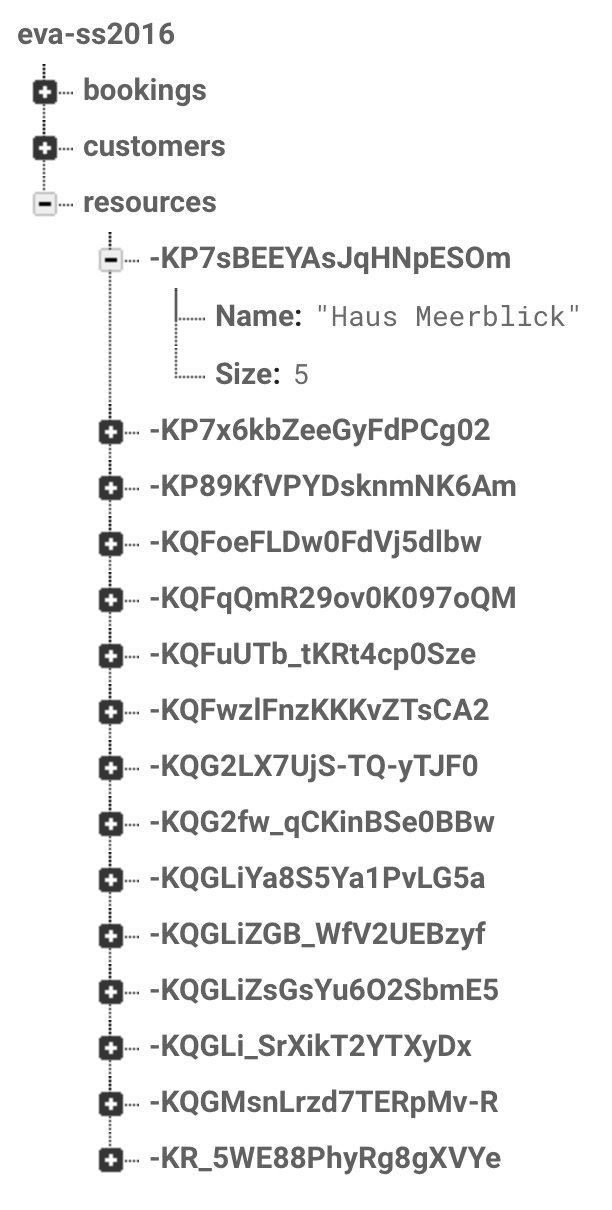
\includegraphics[width=\linewidth]{images/backend_database_resource.png}
        \caption{Datenbank Objekt}
        \label{backend_database_resource}
    \end{minipage}
\end{figure}

Jede Gruppe kann beliebig viele Untergruppen oder Objekte besitzen. Dabei gibt es keine Einschränkungen.\\
Die Daten in den Objekten sind in der JSON-typischen Key:Value-Notation abgelegt.
Identifiziert werden die Objekte über einzigartigen Schlüssel, die als ID fungieren.
Über diese Schlüssel lassen sich später in der Anwendung einzelne Objekte direkt abfragen.
Weiterhin können über diese Keys Beziehungen zu anderen JSON-Objekten aufgebaut werden.
Behandelt werden diese Schlüssel wie Zeichenketten und erfahren somit keiner speziellen Behandlung sofern sie als Werte eines JSON-Objektes abgelegt sind.

\section{Zugriffsverwaltung}
Firebase bietet dem Administrator sehr flexible Zugriffsregeln, mit welchen die exakte Steuerung von Lese- und Schreibzugriffen möglich ist.
Die Ausgangskonfiguration beschränkt das Lesen und Schreiben von Datensätzen auf angemeldete Benutzer. Auf die Möglichkeiten derAuthentifizierung wird in dem Kapitel \ref{chap_auth} eingegangen.\\
Wie die Organisation der Daten in der Datenbank im JSON-Format angelegt ist, werden auch die Regeln als JSON-Notation hinterlegt.
       
\begin{lstlisting}[language=JSON, label=code_AccessRuleDatabase, caption=Beispiel-Konfiguration für Datenbankzugriffe]
		{
         "rules": {
           ".read": "auth != null",
           ".write": "auth != null"
         }
  		}
\end{lstlisting}

Der hier dargestellte Konfigurationsabschnitt zeigt die Regeln für den Lese- und Schreibzugriff auf die gesamte Datenbank. Demnach dürfen nur angemeldete Benutzer lesen und schreiben. Firebase ermöglicht es, für jede Gruppe eine separate Konfiguration zu generieren.
Entscheidend dafür, ob Daten gelesen oder geschrieben werden dürfen ist das Ergebnis des Ausdrucks bei \texttt{.read} und \texttt{.write}. Diese müssen jeweils bei ihrer Ausführung zu einem boolschen Wert evaluieren. Dabei können diese Regeln eine beliebige
Komplexität aufweisen.
In der vorliegenden Anwendung wurde auf eine komplexe und spezifische Konfiguration verzichtet, da der Anwendungsfall keine spezielle Behandlung von verschiedenen Benutzern fordert.
Alle Datensätze können nur von authentifizierten Benutzern gelesen und geschrieben werden.

\section{Lesen, Schreiben, Echtzeit-Synchronisation}
Der entscheidende Punkt bei der Auswahl der Backend-Platform war der Aspekt der Echtzeit-Synchronisation der Datenbank zwischen den angemeldeten Clients.
Um eine Echtzeit-Anwendung zu realisieren, sollten Daten, die bei Client A generiert, verändert oder gelöscht wurden, bei Client B ohne ein Neuladen der gesamten Anwendung aktualisiert werden.\\
Diese Synchronisation wird von Firebase durch die Verwendung der Web-Socket-Technologie ermöglicht. Technisch gesehen basiert dies auf dem Austausch von Nachrichten. Dabei baut die Anwendung eine konstante Verbindung
zu dem Firebase-Server auf. Sobald eine Daten-Transaktion abgeschlossen ist, sendet Firebase eine Nachricht an alle verbundenen Clients. Bei der Entwicklung kann der Entwickler entscheiden, ob er auf etwaige Nachrichten reagieren möchte.
Wie dieses Feature in die entwickelte Anwendung integriert wurde, wird im Kapitel \ref{subchap_coll} Collections genauer erläutert.

\section{Authentifizierung}
\label{chap_auth}
Bei fast jeder zu entwickelnden Anwendung steht das Thema Nutzer-Authentifizierung auf dem Plan. Standardmäßig erfolgen Implementierungen, die Benutzer mit Hilfe von E-Mail Adresse /Benutzernamen und Passwort authentifizieren.
Leider kann es hierbei immer wieder zu Fehlern in der Entwicklung oder im Design kommen, sodass es unter Umständen möglich ist, Zugang zu gesperrten Bereichen oder Daten zu erlangen.
Um dem Entwickler einerseits dieses Risiko zu nehmen und andererseits erheblichen Implementierungs-Aufwand zu ersparen, bietet Firebase auch einen Auhentifizierungs-Service an.
Per Standard ist das E-Mail-Passwort-Verfahren aktiviert. Zudem bietet Firebase auch die Authentifizierung mit Hilfe von Accounts von Facebook, Google, Twitter und GitHub an. Dabei werden OAuth 2.0 und OpenID Connect verwendet. Weiterhin lassen sich
beliebig viele weitere OAuth-Services hinzufügen.\\

In der vorliegenden Anwendung wurde das E-Mail-Passwort-Verfahren verwendet, da analog zum Zugriffsschutz auch hier nur ausgewählte Benutzer Zugriff auf die Anwendung erhalten und somit keine Authentifizierung über weitere Dienste nötig sind.

\begin{figure}[H]
\centering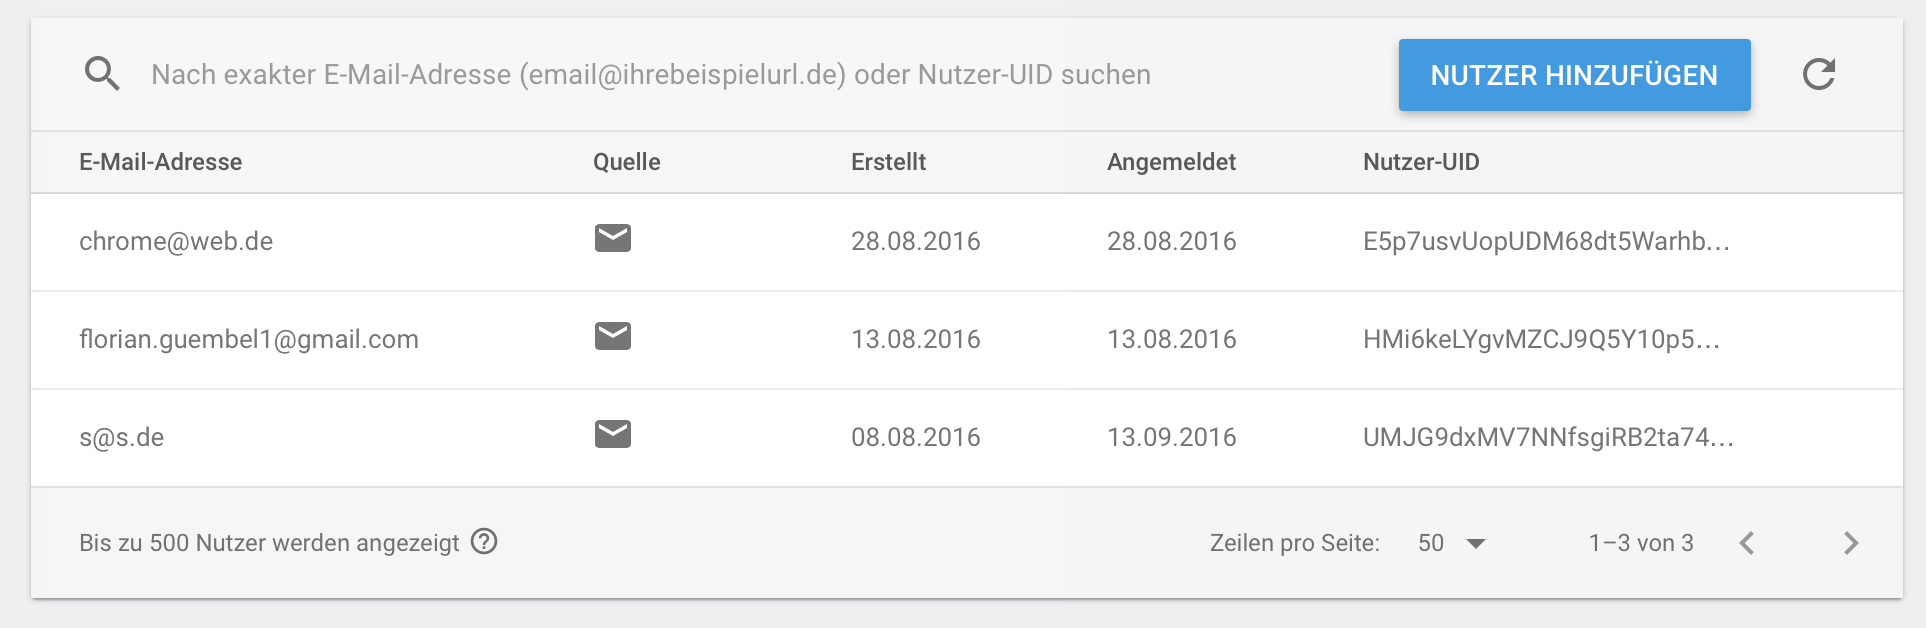
\includegraphics[width=1\textwidth]{images/backend_authentication.png}
\caption{Tabelle mit Email und Password}
\label{backend_authentication}
\end{figure}

Wie diese Anmeldung in der Anwendung abläuft, wird im entsprechenden Kapitel \ref{chap_frontend}  im Bereich Login erläutert.

\section{Weitere Firebase-Funktionen}
Neben den bereits beschriebenen Funktionen stellt Firebase zusätzlich Hosting und Datenspeicher, sowie Cloud Messaging, Analytics und Monetarisierungs-Optionen zur Verfügung.
Zudem bietet Firebase sehr gute Vorraussetzungen für schnell wachsende Anwendungen, da über die Web-Konsole schnell und einfach Kapazitäten angefordert werden können.